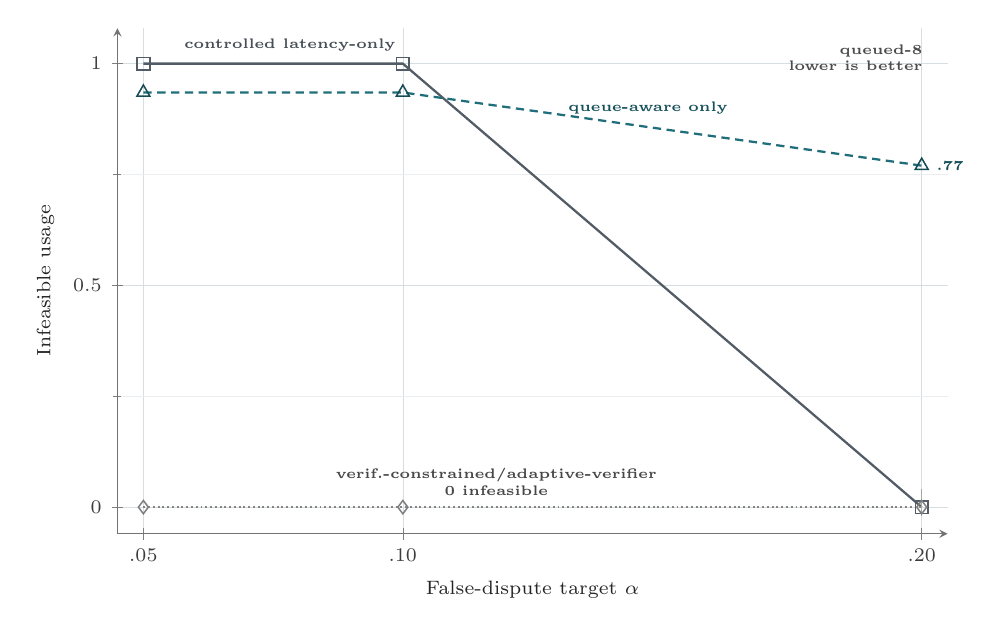
\begin{tikzpicture}
\definecolor{veAlphaTeal}{HTML}{1F6E7A}
\definecolor{veAlphaSlate}{HTML}{525C66}
\definecolor{veAlphaGrid}{HTML}{D7DEE2}
\begin{axis}[
	width=\linewidth,
	height=0.66\linewidth,
	xmin=0.045,
	xmax=0.205,
	ymin=-0.06,
	ymax=1.08,
	axis lines=left,
	axis line style={black!55,line width=0.35pt},
	grid=both,
	major grid style={veAlphaGrid,line width=0.22pt},
	minor grid style={veAlphaGrid!50,line width=0.16pt},
	minor x tick num=1,
	minor y tick num=1,
	xlabel={False-dispute target $\alpha$},
	ylabel={Infeasible usage},
	xlabel style={font=\scriptsize,text=black!85},
	ylabel style={font=\scriptsize,text=black!85},
	tick label style={font=\scriptsize,text=black!76},
	xtick={0.05,0.10,0.20},
	xticklabels={.05,.10,.20},
	ytick={0,0.5,1.0},
	enlarge x limits=false,
	clip=false,
]
\addplot+[mark=square,mark size=2.3pt,line width=0.82pt,
	draw=veAlphaSlate,
	mark options={solid,draw=veAlphaSlate,fill=white,line width=0.55pt}]
	coordinates {(0.05,1.0) (0.10,1.0) (0.20,0.0)};
\node[anchor=south west,font=\tiny\bfseries,text=veAlphaSlate!85!black,align=left]
	at (axis cs:0.056,1.005) {controlled latency-only};

\addplot+[mark=triangle,mark size=2.7pt,line width=0.82pt,
	draw=veAlphaTeal,densely dashed,
	mark options={solid,draw=veAlphaTeal!70!black,fill=white,line width=0.55pt}]
	coordinates {(0.05,0.935) (0.10,0.935) (0.20,0.770)};
\node[anchor=west,font=\tiny\bfseries,text=veAlphaTeal!75!black,align=left]
	at (axis cs:0.13,0.90) {queue-aware only};
\node[anchor=west,font=\tiny\bfseries,text=veAlphaTeal!75!black]
	at (axis cs:0.201,0.770) {.77};

\addplot+[mark=diamond,mark size=2.4pt,line width=0.72pt,
	draw=black!48,densely dotted,
	mark options={solid,draw=black!50,fill=white,line width=0.55pt}]
	coordinates {(0.05,0.0) (0.10,0.0) (0.20,0.0)};
\node[anchor=south,font=\tiny\bfseries,text=black!72,align=center]
	at (axis cs:0.118,0.005) {verif.-constrained/adaptive-verifier\\0 infeasible};

\draw[black!35,line width=0.25pt]
	(axis cs:0.20,-0.02) -- (axis cs:0.20,0.04);
\node[anchor=north east,font=\tiny\bfseries,text=black!70,align=right]
	at (axis cs:0.202,1.065) {queued-8\\lower is better};
\end{axis}
\end{tikzpicture}
